\chapter{سوخت \lr{LPG}}
\section{ مقدمه و اهمیت \lr{LPG} در حمل و نقل دریایی}
تا دسامبر ۲۰۲۳، تعداد ۱۶۴۴ کشتی حامل
 \lr{LPG (LPGC)}
 وجود داشت که از میان آن‌ها، ۲۰۴ کشتی، بر اساس مدل موتور اصلی نصب‌شده، قابلیت تبدیل به سوخت 
 \lr{LPG }
 را داشتند. این تغییر امکان بهره‌برداری از محموله کشتی‌ها و زیرساخت‌های موجود را فراهم کرده و هزینه‌های عملیاتی آن‌ها را به حداقل می‌رساند. 
به عنوان یک سوخت 
\lr{LPG} 
منحصر به فرد هست،‌ زمانی که از کربن‌‌زدایی در کشتی صحبت می‌کنیم نقش مهم و در حال رشدی 
\lr{LPG}
بازی می‌کند.
\lr{LPG} 
عمدتاً از پروپان و بوتان تشکیل شده که تفاوت‌های جزئی شیمیایی آن‌ها باعث کاربردهای خاص می‌شود.
\lr{LPG}
می‌تواند تحت فشار متوسط در دمای معمول مایع شود، که حمل‌ونقل و ذخیره‌سازی آن را آسان‌تر از سایر سوخت‌های گازی می‌کند.
سوخت 
\lr{LPG} 
به صورت مایع حمل و نگهداری می‌شود، اما به صورت گاز مصرف می‌شود، در حالیکه می‌تواند حمل و نقل دریایی تمیزتر به نسبت  بسیاری از جایگزین‌های موجود در حال حاضر ارائه دهد.

سفارشات کشتی‌های با سوخت 
\lr{LPG}
 رکورد شکن شده است، به طور مثال کشتی‌های
\lr{117 VLGC}
  سفارش داده شده یا در حال ساخت با
\lr{LPG}
   حرکت می‌کنند. و پیش‌بینی می‌شود که 86 درصد از این نوع کشتی‌های  
     جدیدی که در سال‌های آینده وارد بازار می‌شوند، قابلیت کار با 
\lr{LPG}
    را داشته باشند. اگرچه 
 \lr{LPG} 
    در حال حاضر یک سوخت محبوب برای حامل های گاز بزرگ است، این بخش تنها 8 درصد از آلاینده های حمل و نقل را به خود اختصاص می‌دهد و 92 درصد آلاینده‌ها را بقیه کشتی‌ها به جا می‌گذارند. تبدیل این کشتی ها یک فرصت عالی برای کاهش انتشار گازهای گلخانه‌ای جهانی است.
جهان ما به طور فزاینده‌ای به سمت کربن کم‌تر حرکت می‌کند و همه بخش‌های اقتصاد باید به مسئله انتشار گازهای گلخانه‌ای بپردازند.
\newpage

در بخش کشتیرانی،
دلایل استفاده از این سوخت به شرح زیر هست:
\begin{enumerate}
	\item 
	توسعه 
	\lr{LPG}
	 به عنوان سوخت دریایی به گسترش فناوری‌های کاهش کربن وابسته است، و پیش‌بینی می‌شود،
	  \lr{rLPG }
	  \LTRfootnote{Refrigerated Liquefied Petroleum Gas}
	  تا سال 2050 تا 50 درصد تقاضای جهانی را پوشش دهد.
	\item 
	\lr{LPG}
	 با استانداردهای زیست‌محیطی فعلی از جمله \textbf{محدودیت گوگرد} سازمان بین‌المللی دریانوردی 
	 \lr{IMO}
	  مطابقت دارد.
	\item 
	\lr{LPG} 
	دارای شبکه حمل‌ونقل گسترده‌ای است که شامل بیش از 1600 کشتی حامل 
	\lr{LPG}
	 و بیش از 1000 تأسیسات ذخیره‌سازی است.
	\item  
	می‌تواند عملکرد زیست‌محیطی بخش کشتیرانی را به سرعت بهبود بخشد.
	\item 
	انتشار گازهای مضر آن کم و هزینه آن، مقرون‌به‌صرفه است که به بهبود محیط‌زیست کمک می‌کند.
	\item 
	\lr{LPG}
	 انعطاف‌پذیر است و زنجیره‌های تأمین آن در سراسر جهان موجود است، که باعث می‌شود زیرساخت‌های سوخت‌رسانی راحت‌تر از بسیاری از سوخت‌های جایگزین دیگر پیاده‌سازی شود.
	 \item 
	 برای سیستم‌های پیشران مبتنی بر
	  \lr{LPG}
هیچ محدودیت یا مانع فناورانه‌ای وجود ندارد.
	
	  \lr{LPG}
	  به فناوری جدید یا پیشرفته نیاز ندارد و آماده بهره‌برداری است.
	 \item 
	 چه برای بزرگ‌ترین کشتی‌های جهان و چه برای کوچک‌ترین موتورهای قایق،
	  \lr{LPG} 
	  امروز یک سوخت کم‌کربن و کم‌انتشار ارائه می‌دهد، و با معرفی 
	  \lr{LPG} 
	  تجدیدپذیر، کربن‌زدایی کم‌هزینه در آینده امکان‌پذیر می‌شود.
\end{enumerate}
\cite{LR_LPG}
	 
\newpage

\begin{table}[h!]
	\centering
	\caption{مشخصات سوخت \lr{LPG}}
	\label{dsd}
	\begin{tabular}{|m{2cm}|m{12cm}|}
		\hline
		\textbf{مشخصه} & \textbf{توضیحات} \\
		\hline
		دمای جوش   & $-42$ درجه (پروپان خالص) و $-0.5$ درجه (بوتان خالص) \\
		فشار بخار & $1.8$ بار (بوتان خالص) تا $7.3$ بار (پروپان خالص) در دمای 15 درجه\\
		 چگالی & $1.89$ کیلوگرم بر متر مکعب (پروپان خالص) تا $2.54$ کیلوگرم بر متر مکعب (بوتان خالص) در دمای $15$ ‌درجه \\
		حداقل انرژی احتراق & $ 0.25 mj$\\
		چگالی انرژی حجمی &  $  26.5MJ/L $   \\
		نسبت اندازه مخزن & $1.5$  \\
		\hline
	\end{tabular}
\end{table}

\section{اثرات زیست محیطی}
\section{تکنولوژی‌های مرتبط با \lr{LPG}}
\subsection{تکنولوژی تولید}
\subsection{تکنولوژی استفاده در کشتی}
\subsection{ایمنی و الزامات فنی }
ذخیره‌سازی، استفاده و حمل‌ونقل
 \lr{LPG}
 خطرات بالقوه‌ای را به همراه دارد که باید در تمامی سناریوهای صنعتی کاهش یابد. در زمینه سوخت دریایی، برای مقابله با این خطرات، اجرای تدابیری در طراحی و ساخت کشتی، تنظیمات ماشین‌آلات و فناوری‌ها، فناوری‌های سوخت‌رسانی، رویه‌های داخلی کشتی و آموزش خدمه ضروری است.
\subsubsection{سنگینی نسبت به هوا}
\lr{LPG}
به صورت گازی تقریباً دو برابر سنگین‌تر از هوا است. این ویژگی باعث می‌شود که در سطوح پایین‌تر جمع شود و خطراتی را در مکان‌های بسته یا گودال‌ها ایجاد کند.تهویه مناسب در سطوح پایین و فضاهای بسته الزامی است.
همچنین استفاده از آشکارسازهای گاز در نزدیکی زمین برای شناسایی نشت گاز الزامی هست.
\subsubsection{مخلوط قابل اشتعال  با هوا}
\lr{LPG}
در غلظت 2 تا 10 درصد با هوا مخلوط قابل اشتعالی تشکیل می‌دهد. در صورت ذخیره یا استفاده نادرست، خطر آتش‌سوزی و انفجار وجود دارد.دوری از منابع گرما، جرقه و شعله باز.
استفاده از تجهیزات ضد انفجار در محل ذخیره یا استفاده.
\subsubsection{تأثیرات استنشاق در غلظت‌های بالا}
در غلظت‌های بسیار بالا، 
\lr{LPG}
 می‌تواند اثرات بی‌هوشی و خفگی داشته باشد زیرا اکسیژن موجود در هوا را رقیق می‌کند.اطمینان از وجود تهویه کافی در فضاهای بسته.
 استفاده از ماسک‌های تنفسی مناسب در شرایط اضطراری.
\subsubsection{سوختگی‌های ناشی از مایع}
 مایع به دلیل تبخیر سریع باعث سوختگی شدید سرد می‌شود. همچنین، تبخیر می‌تواند تجهیزات را به حدی سرد کند که خطر سوختگی را افزایش دهد.
 استفاده از دستکش و لباس‌های محافظ در هنگام کار با 
 \lr{LPG}
  مایع.
 عایق‌کاری مناسب تجهیزات برای جلوگیری از تماس مستقیم.
\subsubsection{احتراق مخلوط بخار/هوا در اثر نشت}
مخلوط بخار 
\lr{LPG}
و هوا می‌تواند در فاصله‌ای دورتر از نقطه نشت آتش بگیرد و شعله به منبع نشت بازگردد.بررسی منظم و رفع نشتی تجهیزات ذخیره و انتقال \lr{LPG}.
نصب شیرهای خودکار قطع گاز برای جلوگیری از گسترش شعله.
\subsubsection{خطرات مخازن خالی}
مخزن خالی
 \lr{LPG}
  ممکن است همچنان حاوی بخار
\lr{\textbf{LPG}}
تخلیه و تهویه کامل مخازن قبل از انجام هرگونه تعمیرات.
برچسب‌گذاری مخازن برای هشدار به افراد از خطرات احتمالی.
\subsection{سیستم‌های ذخیره‌سازی و مدیریت 
	\lr{LPG} 
	در کشتی‌ها}
سوخت‌رسانی
 \lr{LPG}
  به کشتی‌ها به‌عنوان یک سوخت دریایی مزایا و خطراتی دارد. 
   \lr{LPG}
   در حالت مایع خود قابل اشتعال یا انفجار نیست، نشت آن می‌تواند باعث ایجاد بخارهایی شود که به راحتی با باد پراکنده و در صورت برخورد با منبع حرارتی ممکن است آتش بگیرند. همچنین، نشت
    \lr{LPG}
    روی آب می‌تواند منجر به استخر آتش\LTRfootnote{\lr{pool fire}}
     شود که بسیار داغ‌تر و سریع‌تر از آتش‌های ناشی از نفت یا بنزین می‌سوزد و قابل خاموش شدن نیست. در عملیات سوخت‌رسانی، نشت 
    \lr{LPG}
    می‌تواند خطرات زیادی از جمله آتش‌سوزی یا انفجار در مناطق بندری ایجاد کند. به همین دلیل، تدابیر ایمنی ویژه‌ای مانند استفاده از لوله‌های دو جداره و آشکارسازهای هیدروکربنی برای جلوگیری از نشت و آسیب به کشتی‌ها ضروری است. با این حال، سوخت‌رسانی
     \lr{LPG}
     هنوز چارچوب نظارتی رسمی و دستورالعمل‌های مشخصی ندارد و توسعه این دستورالعمل‌ها می‌تواند به بهبود ایمنی، کارایی و آگاهی محیط‌زیستی کمک کند، مشابه آنچه برای دیگر سوخت‌ها مانند 
     \lr{LNG }
     انجام شده است.
\subsection{ایمنی و الزامات فنی مرتبط با حمل }
برای بهبود ایمنی و کارایی در سوخت‌گیری \lr{LPG}، لازم است استانداردها و مشخصات فنی تجهیزات مانند شیلنگ‌ها، نازل‌ها و شیرآلات تدوین شود و معیارهای عملکرد و الزامات ایمنی آن‌ها تعریف گردد. روال‌هایی برای تست و صدور گواهی تجهیزات سوخت‌گیری ایجاد شده و همراه با مستندات و مواد آموزشی جامع، در اختیار ذینفعان از جمله اپراتورها و خدمه قرار گیرد. پروژه‌های آزمایشی و نمایش‌های عملی به منظور اعتبارسنجی چارچوب‌ها و شناسایی شکاف‌ها یا مشکلات احتمالی اجرا شده و از نتایج آن برای اصلاح رویه‌ها و ارتقای ایمنی استفاده شود.

این فرآیندها تضمین می‌کند که تمامی تجهیزات و عملیات مرتبط با سوخت‌گیری \lr{LPG} مطابق با استانداردهای بین‌المللی بوده و صدور گواهی‌ها به ایمنی جهانی کمک کند.
\\
فرآیند سوخت‌گیری در سه مرحله انجام می‌شود.
\subsubsection{مرحله قبل از سوخت‌گیری }
مرحله پیش از سوخت‌گیری 
\LTRfootnote{\lr{Before bunkering}}
	 از سفارش سوخت آغاز شده و با شروع فرآیند سوخت‌گیری خاتمه می‌یابد.  
در این مرحله آمادگی، انجام تمام اقدامات لازم برای اطمینان از انتقال ایمن سوخت بسیار مهم است. این اقدامات شامل موارد زیر می‌شوند:

\begin{itemize}
	\item اطمینان از اینکه تمامی یافته‌های ارزیابی ریسک به درستی مورد توجه قرار گرفته‌اند.
	\item ارزیابی سازگاری بین کشتی دریافت‌کننده سوخت و تأسیسات .
	\item تهیه و توافق بر روی برنامه واکنش اضطراری.
	\item ارائه دستورالعمل‌های ایمنی و آموزش کارکنان .
	\item هماهنگی با نهادهای مسئول برای دریافت مجوزهای لازم.
	\item ارزیابی فرآیندهای مرتبط دیگر، مانند عملیات هم‌زمان \LTRfootnote{\lr{SIMOPS}}.
	\item تعیین جزئیات عملیاتی مانند نرخ انتقال، محدودیت‌های بارگیری،  
	خاموشی اضطراری
	\LTRfootnote{\lr{ESD}}
	، سیستم ایمنی اضطراری
	\LTRfootnote{ERS} 
	و غیره.
	\item تکمیل تمامی چک‌لیست‌های مورد نیاز پیش از سوخت‌گیری.
\end{itemize}

\subsection{مرحله سوخت‌گیری}

فرآیند سوخت‌رسانی
\LTRfootnote{During bunkering}
 با اتصال کشتی دریافت‌کننده به تأسیسات سوخت‌رسانی آغاز می‌شود و با انتقال واقعی سوخت ادامه می‌یابد، و با اقدامات لازم برای بستن ایمن شیر از تأسیسات سوخت‌رسانی خاتمه می‌یابد.  
در طول مرحله سوخت‌گیری، بخش‌های حیاتی سیستم باید به طور مداوم کنترل شوند، از جمله:

\begin{itemize}
	\item سطح مخازن؛
	\item فشار مخازن؛
	\item دمای مخازن؛
	\item نرخ انتقال پمپ؛
	\item نرخ جریان پمپ؛
	\item عملیات سیستم‌های \lr{ESD} و \lr{ERS}؛
	\item تنظیم خطوط پهلوگیری و شیلنگ‌ها؛
	\item نظارت و حفظ سایر جنبه‌های ایمنی، مانند مناطق ایمنی.
\end{itemize}

\subsection{پس‌از سوخت‌گیری}
پس از اتمام سوخت‌گیری
\LTRfootnote{After bunkering}
، باید به نکات زیر توجه شود:
\begin{itemize}
	\item انجام موفقیت‌آمیز فرآیندهای سیستمی ، مانند تبخیر خطوط و خنثی‌سازی گازها در خطوط و شیلنگ‌ها، بدون انتشار گاز به جو.
	\item قطع ایمن ارتباط بین کشتی دریافت‌کننده و تأسیسات سوخت‌رسانی.
	\item جداسازی ایمن کشتی دریافت‌کننده یا کشتی سوخت‌رسان از کشتی دریافت‌کننده و اطلاع‌رسانی به مقامات بندری.
\end{itemize}

\section{الزامات قانونی}
برای کاهش ریسک‌های مرتبط با کشتی، خدمه و محیط زیست، کدهای ایمنی بین‌المللی پیش‌نیازهای لازم برای تجهیزات، ماشین‌آلات و سیستم‌های کشتی را تعیین می‌کنند. این الزامات شامل استانداردهای عملکردی، ارزیابی ریسک، مقررات و نیازمندی‌های عملیاتی است که همراه با آموزش مناسب خدمه، ایمنی عملیات کشتی را تضمین می‌کنند.
\subsection{کد \lr{IGC}}
این کد مرتبط با ساخت و تجهیز کشتی‌هایی که گاز مایع شده را به صورت فله حمل می‌کنند و استفاده از این گازها به‌عنوان سوخت هست.
\subsection{کد \lr{IGF}}
این کد مخصوص کشتی‌های غیرحامل گاز که از گاز یا سوخت‌های با نقطه اشتعال پایین، مانند
\lr{LPG}،
به‌عنوان سوخت استفاده می‌کنند.	

\subsection{استاندارد \lr{MSC.1/Circ.1666}}
استاندارد ایمنی برای کشتی‌هایی که از ال پی جی به‌عنوان سوخت استفاده می‌کنند.
...
\subsection{استاندارد \lr{MSC.1/Circ.1679}}
...راهنمایی‌های موقت برای استفاده از محموله ال پی جی به‌عنوان سوخت.


\section{اقتصاد و بازار \lr{LPG}}
\subsection{چرخه عمر}
دستورالعمل‌های چرخه عمر گازهای گلخانه‌ای 
\LTRfootnote{\lr{LCA}}
 سازمان بین‌المللی دریانوردی  برای سوخت‌های دریایی، شامل 
 \lr{LPG}
 ، ابتدا در نشست 
 \lr{MEPC 80 (MEPC.376(80))}
 تصویب شدند و تمامی مراحل زنجیره تأمین این سوخت را پوشش می‌دهند. در نشست
  \lr{MEPC 81}،
   نسخه
    \lr{2024}
    این دستورالعمل‌ها 
  \lr{  (MEPC.391(81)) }
    با اصلاح عوامل توزیع پیش‌فرض، به‌روزرسانی الگوی عوامل توزیع از چاه به مخزن
    \LTRfootnote{Well-to-Tank}
    \cref{Suplly-Chain}
     و اضافه‌شدن الگوی جدید برای عوامل توزیع از مخزن به مصرف 
\LTRfootnote{Tank-to-Wake}
      بازنگری شد.
 \cite{Comparative-Life-Cycle}
 \begin{figure}[!h]
 	\centering
 	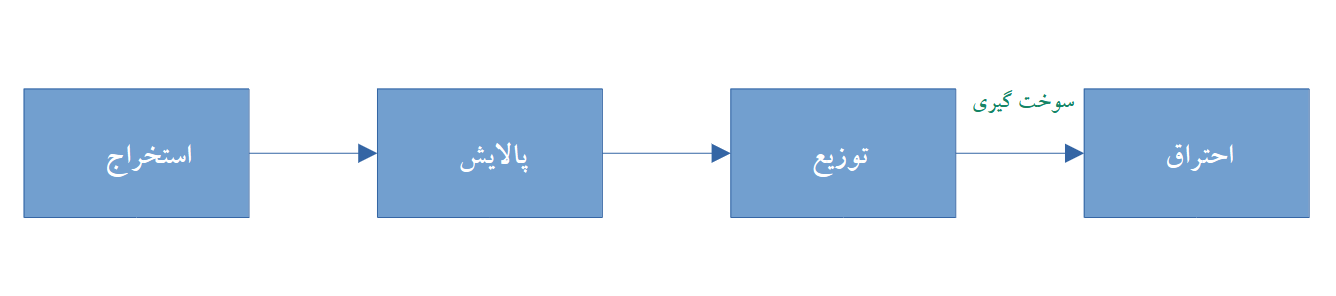
\includegraphics[width=15cm]{Figures/LPG/supply-chain.png}
 	\caption{ زنجیره تأمین سوخت}\label{Suplly-Chain}
 \end{figure}
 
\subsection{تجارت جهانی}
 تقاضای جهانی  
 \lr{LPG }
 در
  \cref{future}
 و تجارت دریایی مرتبط با آن در حال افزایش است. در سال 2022،
  تقاضای جهانی
   \lr{LPG}
    با رشد 
    $\%$5.3
    به رکورد 342 میلیون تن رسید. پیش‌بینی‌ها نشان می‌دهد که حجم تجارت دریایی
    \lr{LPG}
     در سال 2023 حدود 6 میلیون تن افزایش یافته و نسبت به 2022 رشد 5$\%$
   
      داشته است. همچنین، برای سال 2024، رشد
      $\%$3.2
        پیش‌بینی شده و انتظار می‌رود حجم تجارت تا سال 2027 به حدود 142 میلیون تن برسد.
 \begin{figure}[!h]
	\centering
	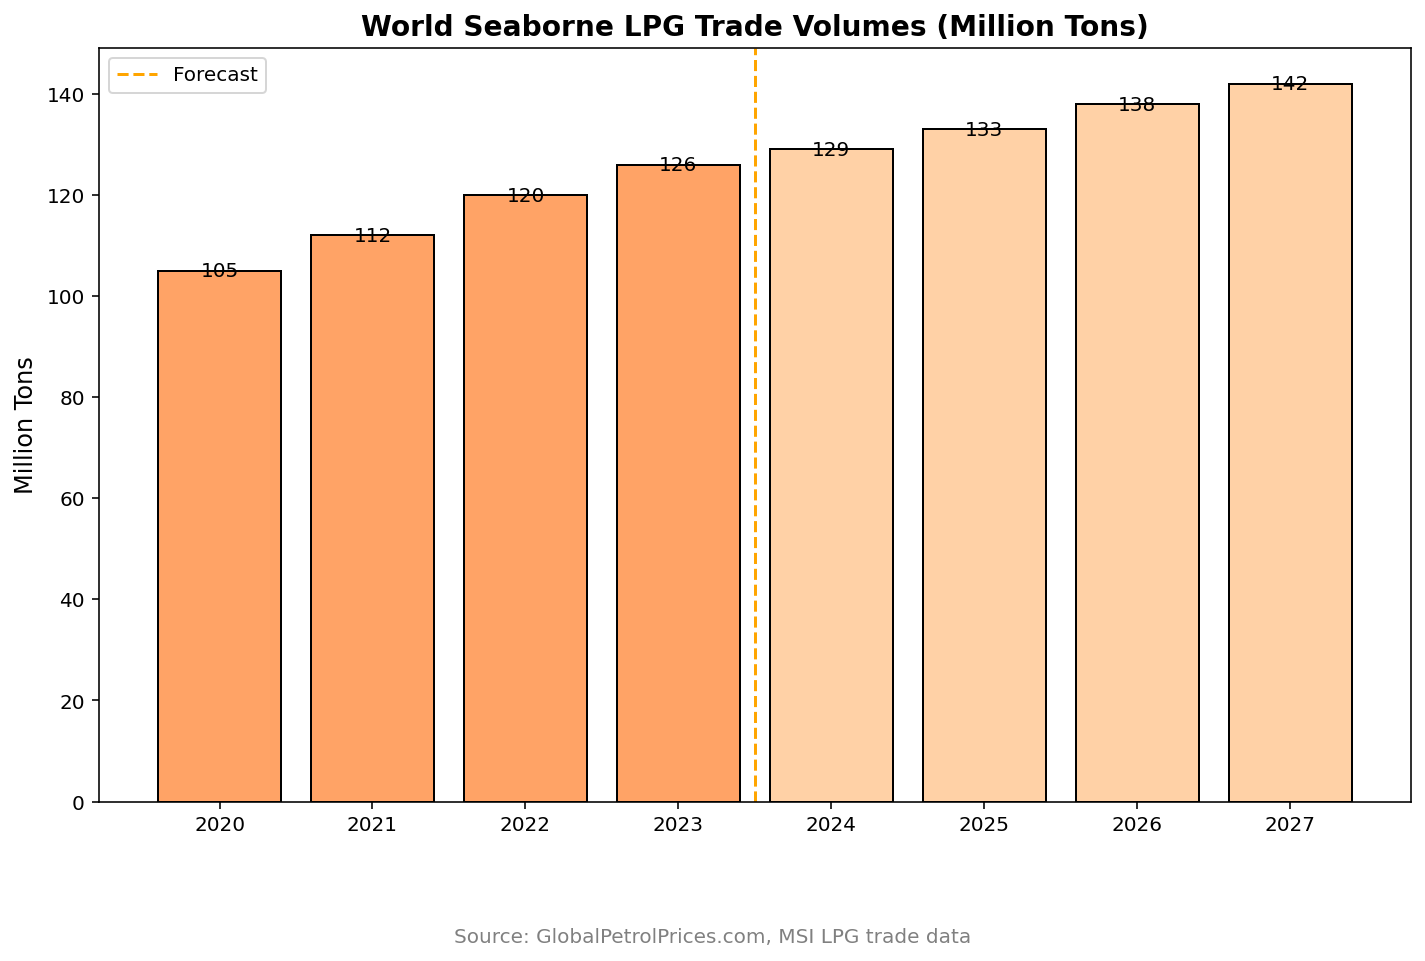
\includegraphics[width=15cm]{Figures/LPG/future.png}
	\caption{ درخواست \lr{LPG}}\label{future}
\end{figure} 
 
\subsection{قیمت سوخت}
استفاده از
 \lr{LPG}
 (گاز مایع) به عنوان سوخت، به‌دلیل قیمت جذاب آن در برخی مناطق مانند ایالات متحده و خلیج فارس، گزینه‌ای اقتصادی برای مالکان و اپراتورها محسوب می‌شود. از نظر هزینه‌های سرمایه‌ای 
 \LTRfootnote{(CAPEX)}،
  \lr{LPG }
 مزایای قابل توجهی نسبت به سایر گزینه‌های سوخت دوگانه 
\LTRfootnote{Dual-Fuel}
  مانند 
  \lr{LNG}
   دارد؛ به‌طوری که ساخت یک کشتی کانتینری ۱۰ هزار 
   \lr{TEU}
   با سوخت 
   \lr{LPG}
    حدود ۱۰۰ میلیون دلار هزینه دارد، یعنی ۲۰$\%$ ارزان‌تر از کشتی مشابه با سوخت 
    \lr{LNG }
    که حدود ۱۲۵ میلیون دلار هزینه می‌برد. همچنین، هزینه تبدیل موتورهای دیزلی به موتورهای دوگانه 
    \lr{LPG }
    (بین ۹.۵ تا ۲۷ میلیون دلار) در مقایسه با تبدیل به
     \lr{LNG}
     (بین ۱۲ تا ۳۳ میلیون دلار) مقرون‌به‌صرفه‌تر است. این عوامل باعث می‌شود.
      \lr{LPG }
      به‌عنوان گزینه‌ای جذاب برای صنعت کشتیرانی مطرح شود.
(\cref{price})
\begin{figure}[!h]
   	\centering
   		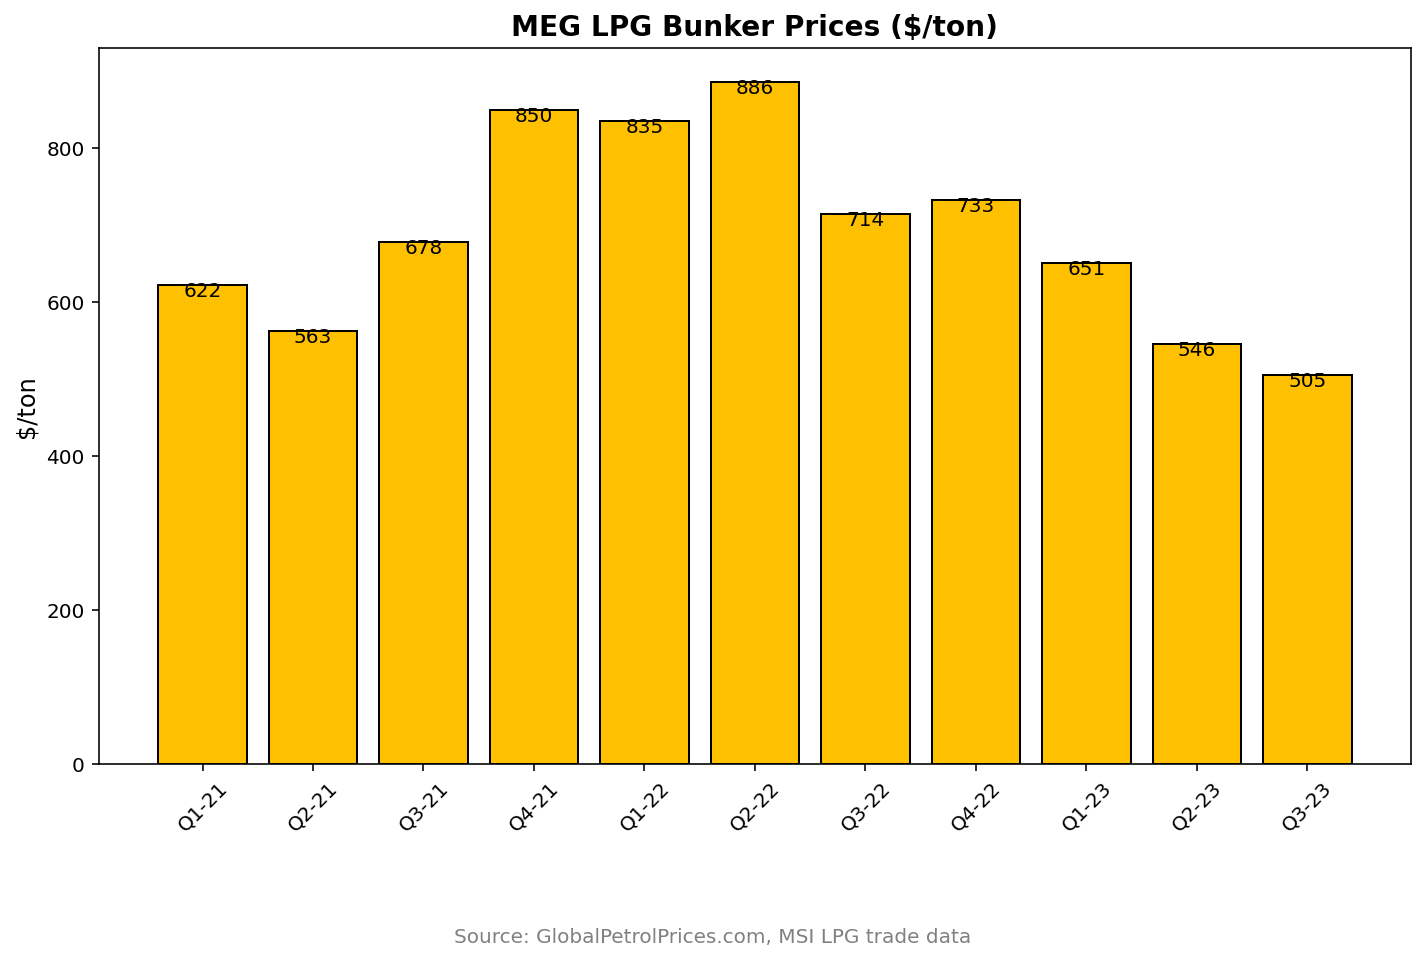
\includegraphics[width=15cm]{Figures/LPG/price.png}
   	\caption{ قیمت سوخت در خلیج فارس}\label{price}
\end{figure}
\\
\\
\subsection{تأمین و نگهداری}
\section{نتیجه‌گیری}
\begin{itemize}
	\item \textbf{مزایای زیست‌محیطی \lr{LPG}:}
	\begin{itemize}
		\item LPG به‌عنوان یک سوخت فسیلی مزیت‌های قابل توجهی در کاهش \textbf{آلودگی هوا} نسبت به سوخت‌های نفتی سنتی (مانند مازوت) دارد.
		\item استفاده از LPG موجب \textbf{کاهش انتشار گازهای گلخانه‌ای} می‌شود، به‌ویژه اگر با فناوری‌های مکملی مانند \textbf{کربن‌گیری در کشتی} همراه شود.
		\item این سوخت می‌تواند با \textbf{مقررات سازمان بین‌المللی دریانوردی (IMO)} درباره کاهش اکسیدهای گوگرد مطابقت داشته باشد و همچنین در بلندمدت با اهداف کربن‌زدایی این سازمان همخوانی داشته باشد.
	\end{itemize}
	
	\item \textbf{پتانسیل LPG برای آینده:}
	\begin{itemize}
		\item استفاده از LPG در بلندمدت به تولید سوخت‌های تجدیدپذیر وابسته است، که انتظار می‌رود با سرعت بالایی افزایش یابد.
		\item با رشد تجارت دریایی و افزایش تقاضا برای LPG، ناوگان جهانی کشتی‌های حمل LPG رشد خواهد کرد و این فرصت برای استفاده از LPG به‌عنوان سوخت افزایش می‌یابد.
		\item زیرساخت‌های حمل‌ونقل، ذخیره‌سازی و استفاده از LPG طی چند دهه به‌خوبی توسعه یافته است.
	\end{itemize}
	
	\item \textbf{چالش‌های موجود:}
	\begin{itemize}
		\item تکنولوژی‌های موتوری برای LPG محدود است. به‌عنوان مثال، هنوز موتور دریایی چهارزمانه‌ای که بتواند از LPG استفاده کند، وجود ندارد، بنابراین موتورهای کمکی کشتی‌ها نیاز به سوخت‌های دیگری برای کربن‌زدایی دارند.
		\item قوانین و چارچوب‌های مقرراتی برای استفاده از LPG به‌عنوان سوخت، خصوصاً در حوزه \textbf{سوخت‌رسانی (bunkering)}، هنوز کامل نیست و فقط راهنماهای اولیه در سطح IMO تدوین شده است.
	\end{itemize}

	\item \textbf{عامل تعیین‌کننده:}
	\begin{itemize}
		\item آینده LPG به‌عنوان یک سوخت مهم در صنعت دریانوردی به سرعت \textbf{کربن‌زدایی تولید LPG} و پیشرفت فناوری‌های مرتبط مانند \textbf{کربن‌گیری} وابسته است.
		\item همچنین LPG ممکن است به‌عنوان یک سوخت \textbf{انتقالی} تا زمان توسعه کامل سوخت‌های بدون کربن یا نزدیک به صفر کربن عمل کند.
	\end{itemize}
\end{itemize}


